\chapter{Student Questionnaire}
\label{appendix:studentquestionnaire}

The questionnaire for accessing the students' opinions regarding EDCAT is shown in Figure~\ref{fig:studentquestionnaire}.

\begin{figure}
\caption{The student questionnaire (continued on next page).}
\label{fig:studentquestionnaire}
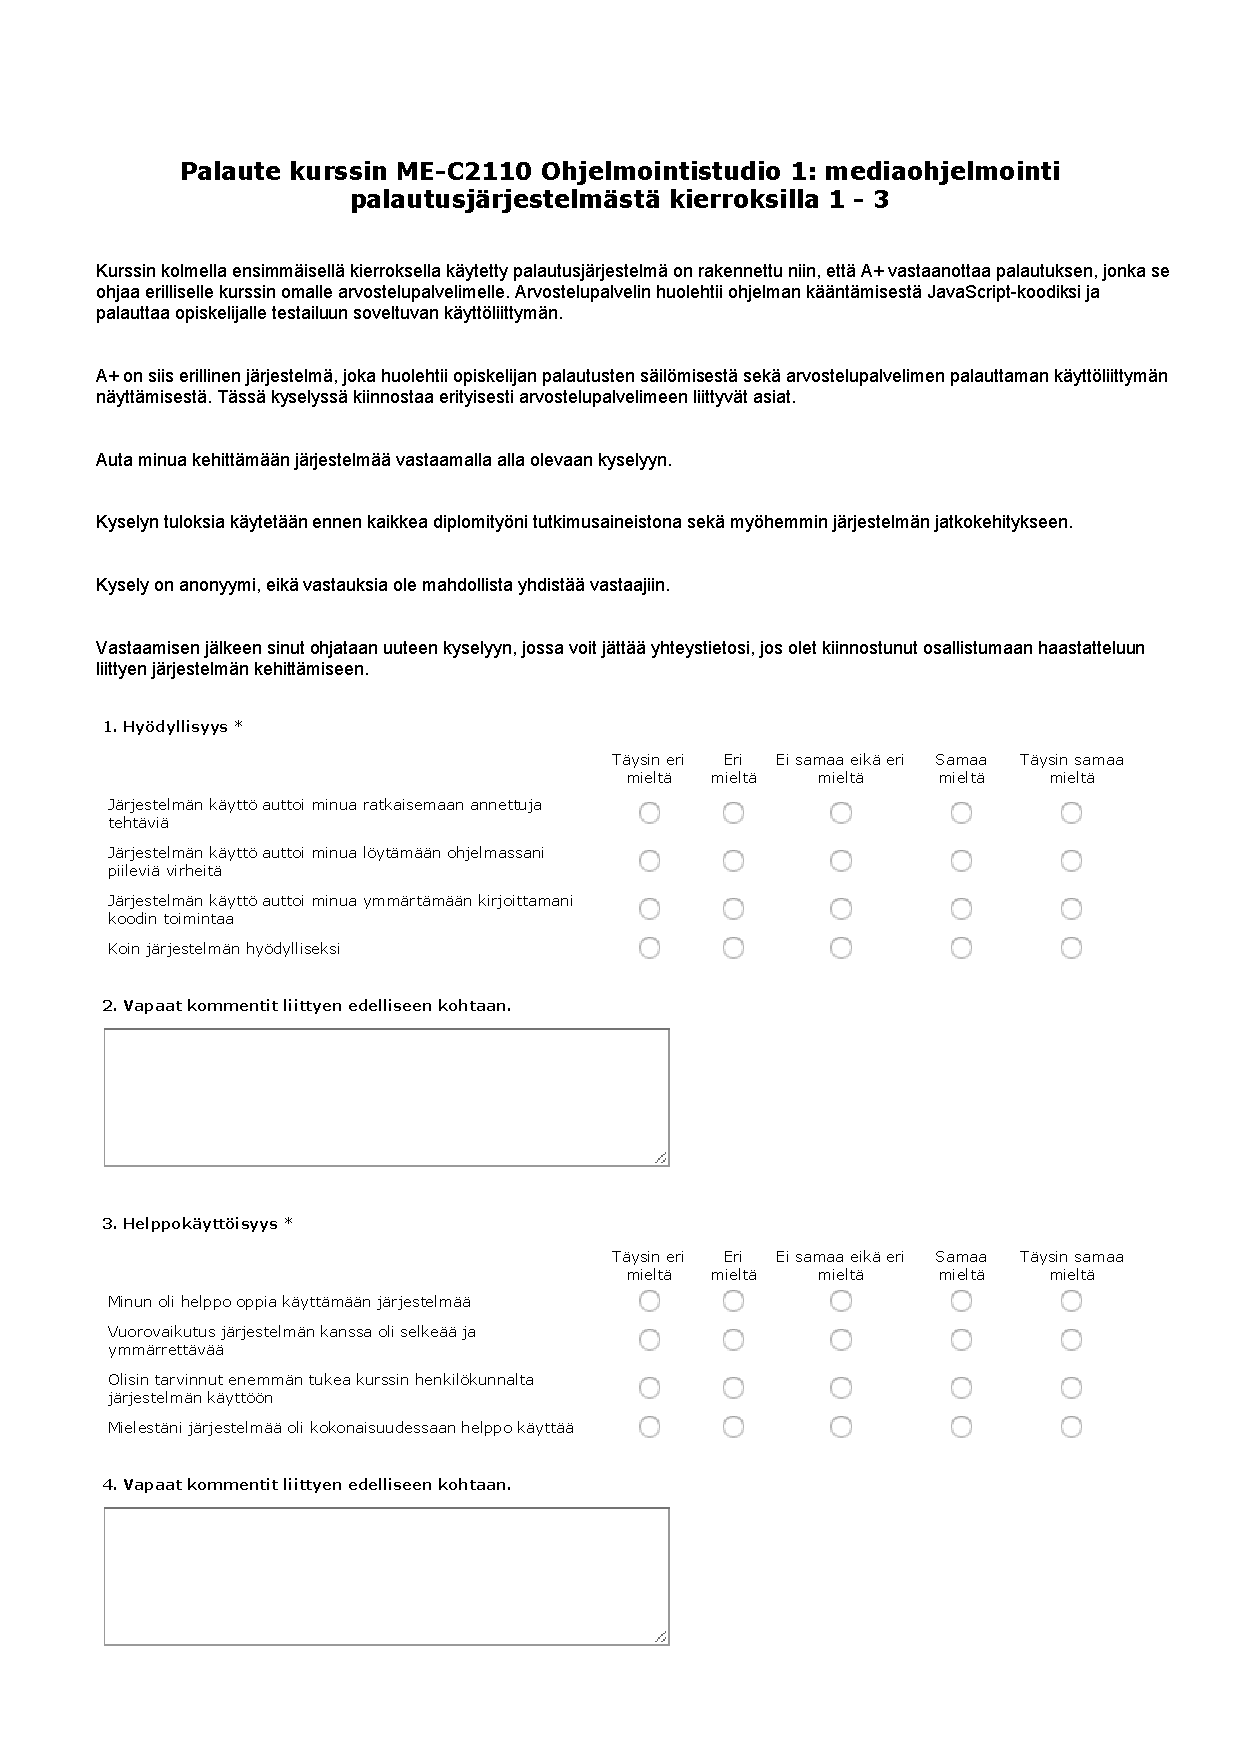
\includegraphics[page=1, width=\textwidth, height=\textheight]{images/kysely-opiskelijat1.pdf}
\end{figure}

\begin{figure}
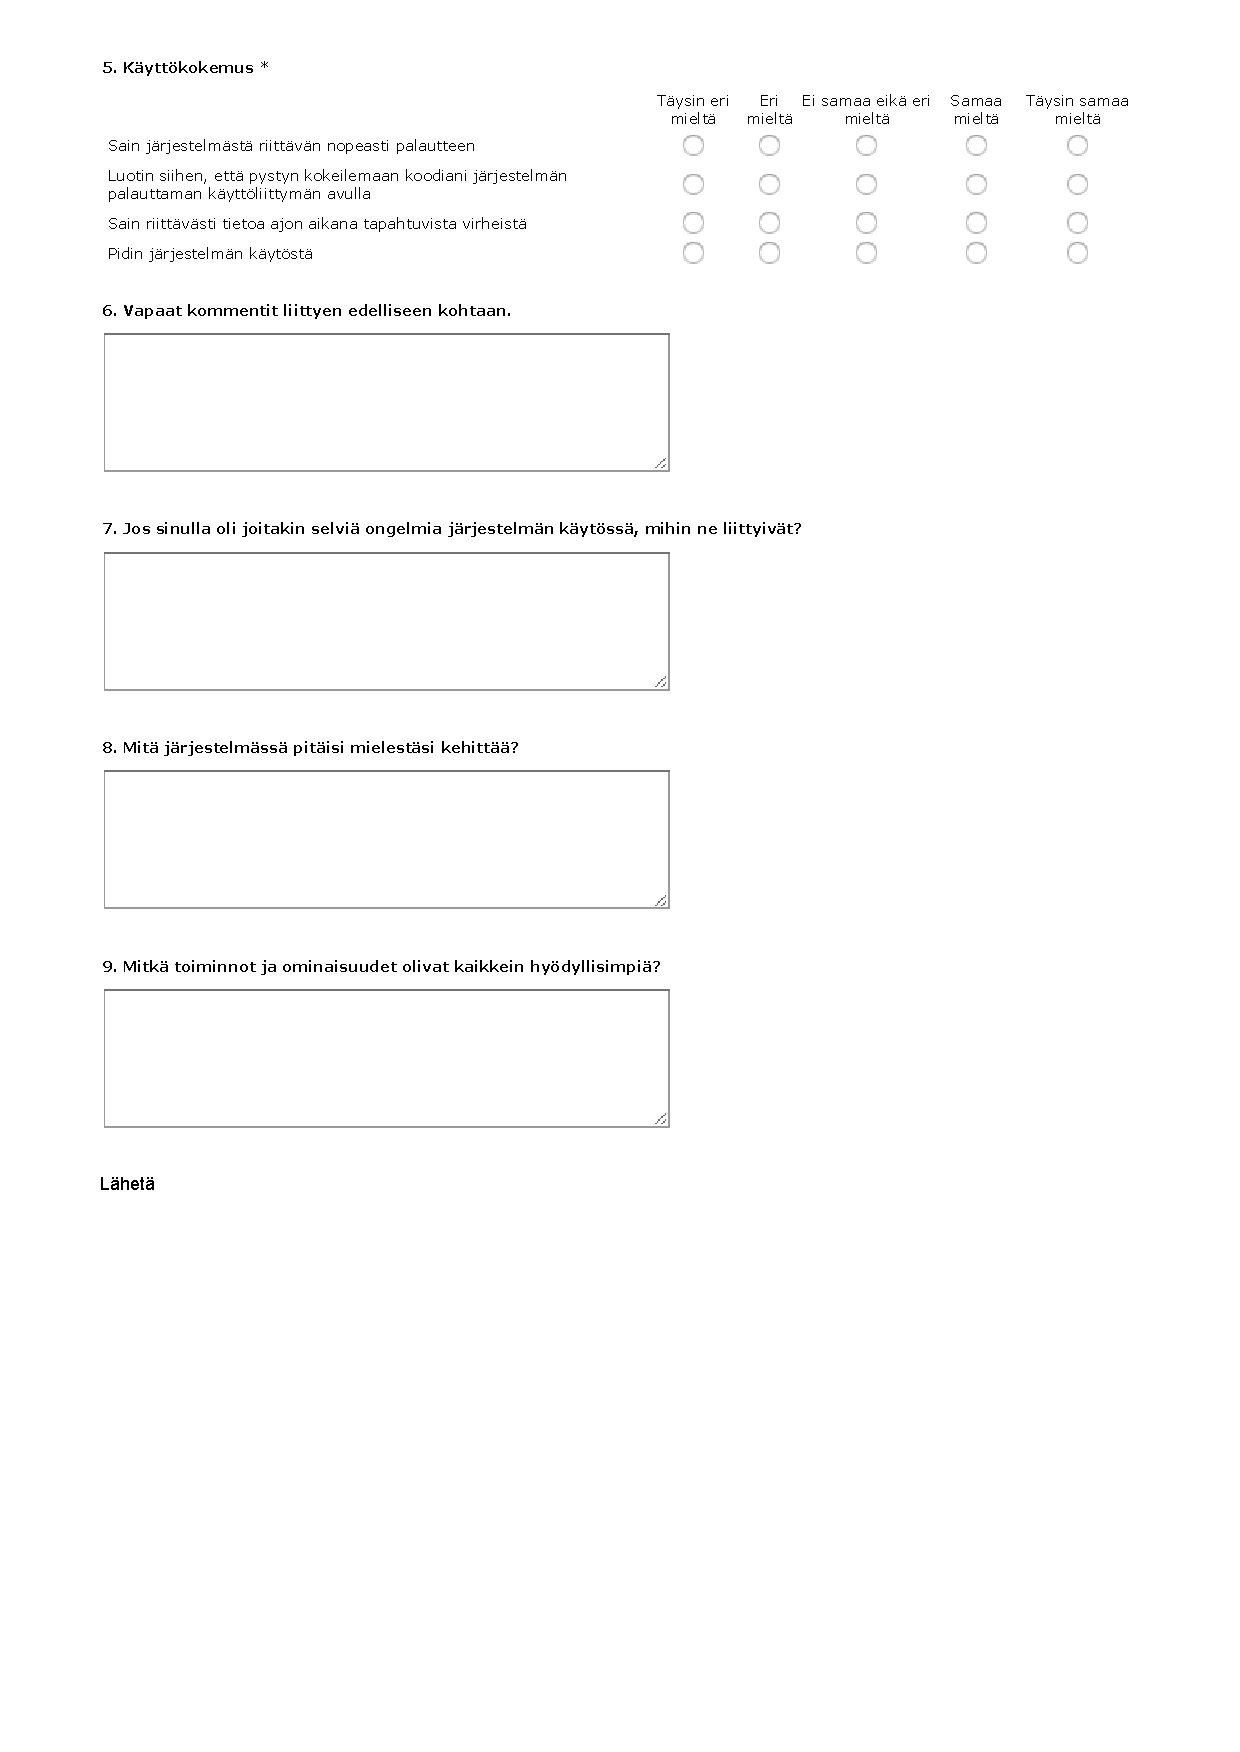
\includegraphics[page=1, width=\textwidth]{images/kysely-opiskelijat2.pdf}
\end{figure}



\chapter{Teaching Assistant Questionnaire}
\label{appendix:TAquestionnaire}

The questionnaire for accessing the teaching assistants' opinions regarding EDCAT is shown in Figure~\ref{fig:TAquestionnaire}.

\begin{figure}
\caption{The teaching assistant questionnaire.}
\label{fig:TAquestionnaire}
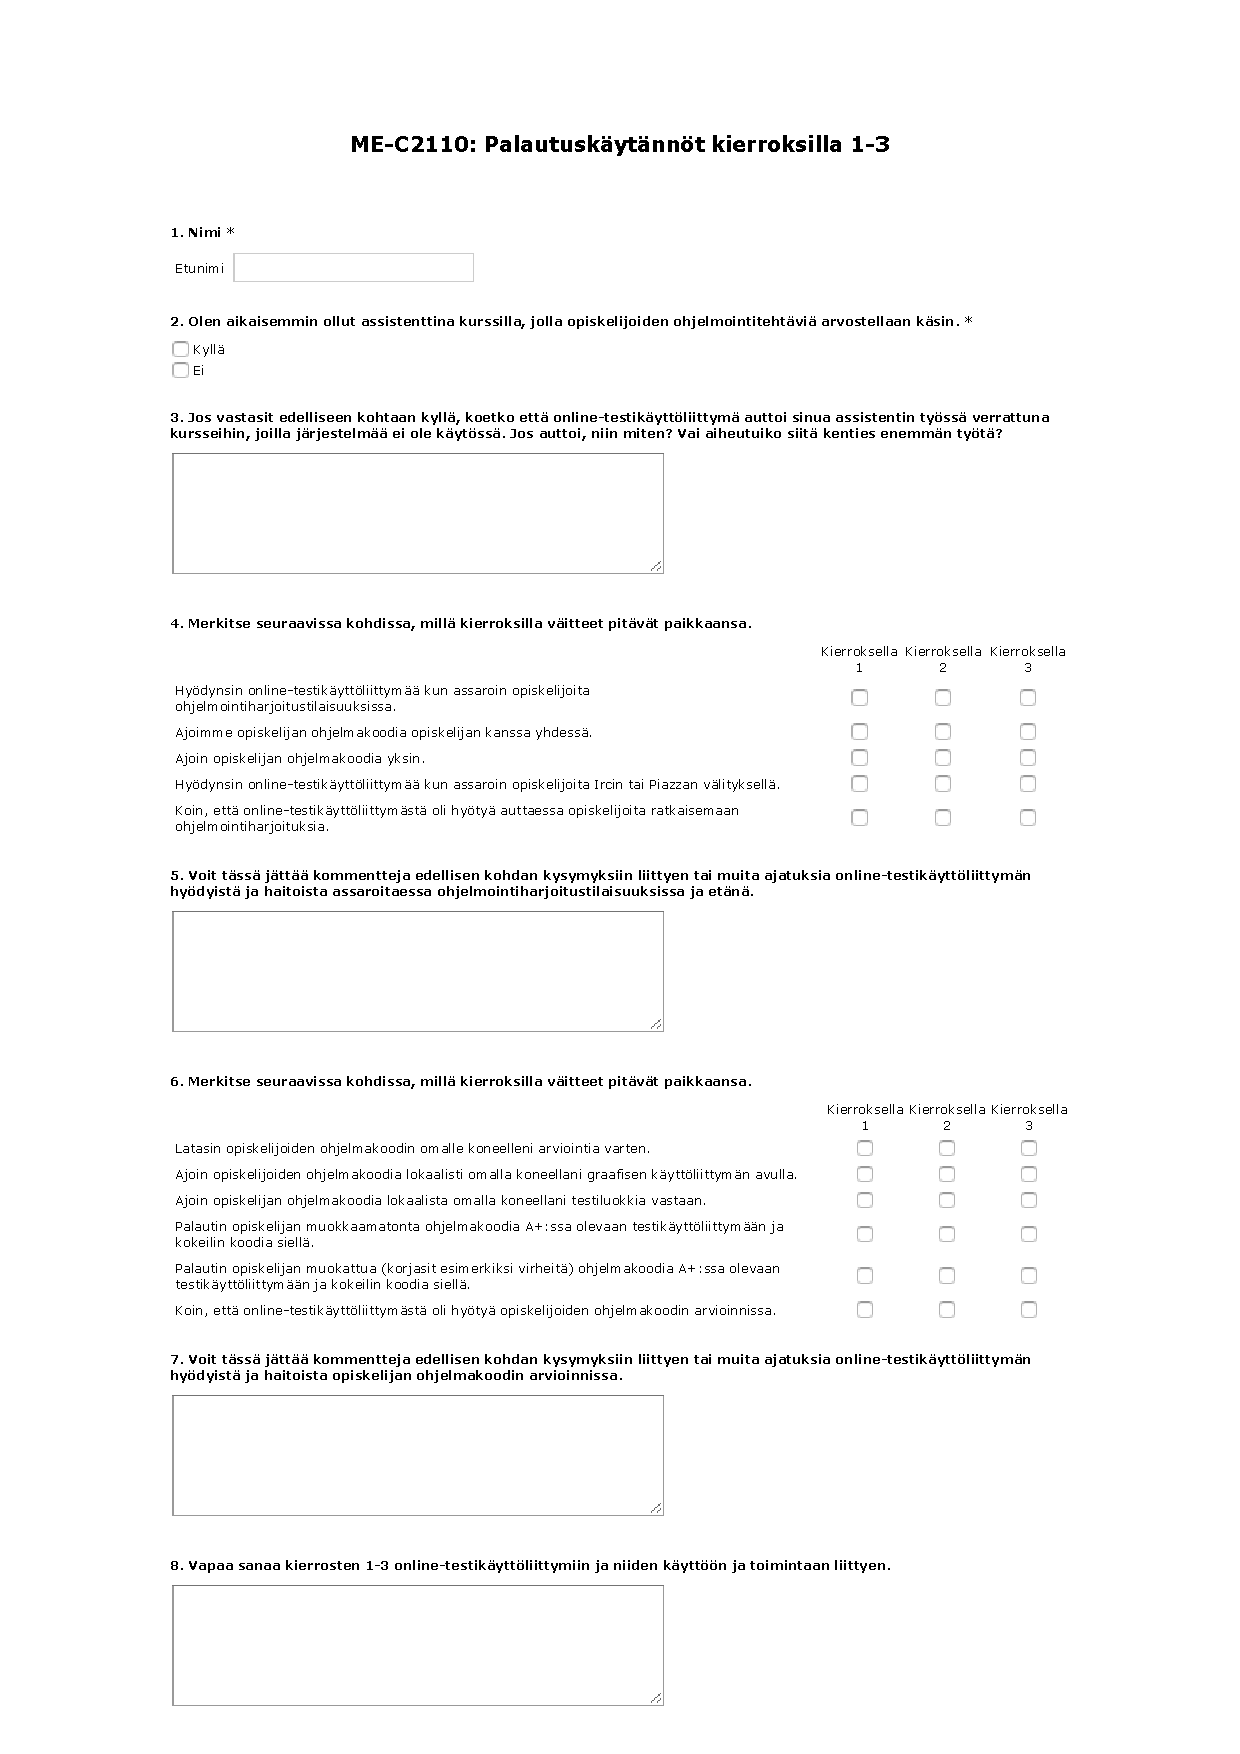
\includegraphics[page=1, width=\textwidth, height=\textheight]{images/kysely-assarit2.pdf}
\end{figure}



\chapter{Further Analysis of Submission Numbers}
\label{appendix:first-vs-number}

Comparison of students' first submission date with the number of submissions the student or student pair used. There is no clear pattern to indicate a reason for why some students used significant amount of submissions or why some did not.

\begin{figure}
	\begin{center}
		\begin{tikzpicture}
	\begin{groupplot}[group style = {group size = 2 by 2, vertical sep=2cm}, grid=both,
										width=0.5*\textwidth, every axis title/.append style={font=\footnotesize,},
										date coordinates in=x, xticklabel={\day.\month.},
										xticklabel style={rotate=45,anchor=north east},
										extra tick style={major grid style=red, xticklabel={\day.\month.}, ytick align=outside},
										tick label style={font=\footnotesize},
										x label style={at={(axis description cs:0.5,-0.5)},anchor=north,font=\footnotesize}]

		\nextgroupplot[	title=(a) Assignment 1.1,
										extra x ticks={2015-10-02 16:00:00, 2015-10-07 16:00:00}, xtick={2015-09-25 16:00:00},
										minor xtick={	2015-09-20 16:00:00, 2015-09-21 16:00:00, 2015-09-22 16:00:00,
																	2015-09-23 16:00:00, 2015-09-24 16:00:00, 2015-09-26 16:00:00,
																	2015-09-27 16:00:00, 2015-09-28 16:00:00, 2015-09-29 16:00:00,
																	2015-09-30 16:00:00, 2015-10-01 16:00:00, 2015-10-03 16:00:00,
																	2015-10-04 16:00:00, 2015-10-05 16:00:00},
										date ZERO=2015-09-20]
	  \addplot+[scatter, only marks, mark=o, scatter src=explicit symbolic,
								scatter/classes={12={mark=diamond,cyan},11.5={mark=diamond,cyan},11={mark=diamond,cyan},
																 10.5={mark=diamond,cyan},10={mark=o,blue},9.5={mark=o,blue},9={mark=o,blue},
																 8.5={mark=o,blue},8={mark=none},7.5={mark=none},7={mark=none},6.5={mark=none},
																 6={mark=none},5.5={mark=none},5={mark=none},4={mark=none},0={mark=none}}]
							table [meta=points, col sep=comma] {data/first-vs-number-1-1.csv};
	  \addplot+[scatter, only marks, mark=o, scatter src=explicit symbolic,
								scatter/classes={12={mark=none},11.5={mark=none},11={mark=none},10.5={mark=none},
																 10={mark=none},9.5={mark=none},9={mark=none},8.5={mark=none},
																 8={mark=star,black},7.5={mark=star,black},7={mark=star,black},
																 6.5={mark=star,black},6={mark=o,orange},5.5={mark=o,orange},5={mark=o,orange},
																 4={mark=o,orange},0={mark=o,red}}]
							table [meta=points, col sep=comma] {data/first-vs-number-1-1.csv};

		\nextgroupplot[	title=(b) Assignment 1.2,
										extra x ticks={2015-10-02 16:00:00, 2015-10-07 16:00:00},
										xtick={2015-09-25 16:00:00, 2015-10-09 16:00:00, 2015-10-16 16:00:00},
										minor xtick={	2015-09-20 16:00:00, 2015-09-21 16:00:00, 2015-09-22 16:00:00,
																	2015-09-23 16:00:00, 2015-09-24 16:00:00, 2015-09-26 16:00:00,
																	2015-09-27 16:00:00, 2015-09-28 16:00:00, 2015-09-29 16:00:00,
																	2015-09-30 16:00:00, 2015-10-01 16:00:00, 2015-10-03 16:00:00,
																	2015-10-04 16:00:00, 2015-10-05 16:00:00, 2015-10-06 16:00:00,
																	2015-10-08 16:00:00, 2015-10-10 16:00:00, 2015-10-11 16:00:00, 
																	2015-10-12 16:00:00, 2015-10-13 16:00:00, 2015-10-14 16:00:00,
																	2015-10-15 16:00:00},
										date ZERO=2015-09-20]
	  \addplot+[scatter, only marks, mark=o, scatter src=explicit symbolic,
								scatter/classes={12={mark=diamond,cyan},11.5={mark=diamond,cyan},11={mark=diamond,cyan},
																 10.5={mark=diamond,cyan},10={mark=o,blue},9.5={mark=o,blue},9={mark=o,blue},
																 8.5={mark=o,blue},8={mark=none},7.5={mark=none},7={mark=none},6.5={mark=none},
																 6={mark=none},5.5={mark=none},5={mark=none},0={mark=none}}]
							table [meta=points, col sep=comma] {data/first-vs-number-1-2.csv};
	  \addplot+[scatter, only marks, mark=o, scatter src=explicit symbolic,
								scatter/classes={12={mark=none},11.5={mark=none},11={mark=none},10.5={mark=none},
																 10={mark=none},9.5={mark=none},9={mark=none},8.5={mark=none},
																 8={mark=star,black},7.5={mark=star,black},7={mark=star,black},
																 6.5={mark=star,black},6={mark=o,orange},5.5={mark=o,orange},5={mark=o,orange},
																 0={mark=o,red}}]
							table [meta=points, col sep=comma] {data/first-vs-number-1-2.csv};

		\nextgroupplot[	title=(c) Assignment 2,
										ylabel=Number of submissions for the Assignment Round,
										every axis y label/.append style={font=\footnotesize, at={(0.0,1.3)}},
										xlabel=The First Submission Date,
										every axis x label/.append style={font=\footnotesize, at={(1.1,-0.2)}},
											extra x ticks={2015-10-16 16:00:00, 2015-10-21 16:00},
											xtick={2015-10-09 16:00:00, 2015-10-23 16:00:00},
											minor xtick={	2015-10-03 16:00:00, 2015-10-04 16:00:00, 2015-10-05 16:00:00,
																		2015-10-06 16:00:00, 2015-10-07 16:00:00, 2015-10-08 16:00:00,
																		2015-10-10 16:00:00, 2015-10-11 16:00:00, 2015-10-12 16:00:00,
																		2015-10-13 16:00:00, 2015-10-14 16:00:00, 2015-10-15 16:00:00,
																		2015-10-17 16:00:00, 2015-10-18 16:00:00, 2015-10-19 16:00:00,
																		2015-10-20 16:00:00, 2015-10-22 16:00:00, 2015-10-24 16:00:00,
																		2015-10-25 16:00:00, 2015-10-26 16:00:00, 2015-10-27 16:00:00,
																		2015-10-28 16:00:00},
											date ZERO=2015-10-03,
											ytick={0,20,40,60,80}]
			\addplot+[scatter, only marks, mark=o, scatter src=explicit symbolic,
								scatter/classes={24={mark=diamond,cyan},23={mark=diamond,cyan},22={mark=diamond,cyan},
																 21={mark=diamond,cyan},20={mark=o,blue},19={mark=o,blue},18={mark=o,blue},
																 17={mark=o,blue},16={mark=none},15={mark=none},14={mark=none},13={mark=none},
																 12={mark=none},11={mark=none},10={mark=none},0={mark=none}}]
							table [meta=points, col sep=comma] {data/first-vs-number-2.csv};
	  \addplot+[scatter, only marks, mark=o, scatter src=explicit symbolic,
								scatter/classes={24={mark=none},23={mark=none},22={mark=none},21={mark=none},
																 20={mark=none},19={mark=none},18={mark=none},17={mark=none},
																 16={mark=star,black},15={mark=star,black},14={mark=star,black},
																 13={mark=star,black},12={mark=*,orange},11={mark=*,orange},10={mark=*,orange},
																 0={mark=o,red}}]
							table [meta=points, col sep=comma] {data/first-vs-number-2.csv};

		\nextgroupplot[ title=(d) Assignment 3,
										extra x ticks={2015-11-06 16:00:00, 2015-11-11 16:00},
										xtick={2015-10-23 16:00:00, 2015-10-30 16:00:00, 2015-11-13 16:00:00},
										minor xtick={ 2015-10-18 16:00:00, 2015-10-19 16:00:00, 2015-10-20 16:00:00,
										  						2015-10-21 16:00:00, 2015-10-22 16:00:00, 2015-10-24 16:00:00,
																	2015-10-25 16:00:00, 2015-10-26 16:00:00, 2015-10-27 16:00:00,
																	2015-10-28 16:00:00, 2015-10-29 16:00:00, 2015-10-30 16:00:00,
																	2015-10-31 16:00:00, 2015-11-01 16:00:00, 2015-11-02 16:00:00,
																	2015-11-03 16:00:00, 2015-11-04 16:00:00, 2015-11-05 16:00:00, 
																	2015-11-07 16:00:00, 2015-11-08 16:00:00, 2015-11-09 16:00:00,
																	2015-11-10 16:00:00, 2015-11-12 16:00:00},
										date ZERO=2015-10-18]
	  \addplot+[scatter, only marks, mark=o, scatter src=explicit symbolic,
								scatter/classes={24={mark=diamond,cyan},23={mark=diamond,cyan},22={mark=diamond,cyan},
																 21={mark=diamond,cyan},20={mark=o,blue},19={mark=o,blue},18={mark=o,blue},
																 17={mark=o,blue},16={mark=none},15={mark=none},14={mark=none},13={mark=none},
																 12={mark=none},11={mark=none},10={mark=none},8={mark=none},0={mark=none}}]
							table [meta=points, col sep=comma] {data/first-vs-number-3.csv};
	  \addplot+[scatter, only marks, mark=o, scatter src=explicit symbolic,
								scatter/classes={24={mark=none},23={mark=none},22={mark=none},21={mark=none},
																 20={mark=none},19={mark=none},18={mark=none},17={mark=none},
																 16={mark=star,black},15={mark=star,black},14={mark=star,black},
																 13={mark=star,black},12={mark=*,orange},11={mark=*,orange},10={mark=*,orange},
																 8={mark=*,orange},0={mark=o,red}}]
							table [meta=points, col sep=comma] {data/first-vs-number-3.csv};

	\end{groupplot}
	\begin{customlegend}[
		legend entries={\textless10 points, 12-10 points, 16-13 points, 20-17 points, \textgreater20 points},
		legend style={at={(5.0,-9.0)}, anchor=north, font=\footnotesize},
		legend columns=5,
		/tikz/every even column/.append style={column sep=0.7cm}]
			\addlegendimage{only marks, mark=o,red}
			\addlegendimage{only marks, mark=*,orange}
			\addlegendimage{only marks, mark=star,black}
			\addlegendimage{only marks, mark=o,blue}
			\addlegendimage{only marks, mark=diamond,cyan}
	\end{customlegend}
\end{tikzpicture}
	\end{center}
	\caption[asdf]{Students' first submissions compared with the number of submissions for the assignment
  							 round. The vertical lines indicate the deadline and the late submission
								 deadline. In the first assignment round the markers respond to legend's markers divided by two.}
	\label{figure:first-vs-number}
\end{figure}
